\documentclass[a4paper, 12pt]{article}
\usepackage[a4paper,top=1.5cm, bottom=1.5cm, left=1cm, right=1cm]{geometry}

% Работа с русским языком
\usepackage[utf8]{inputenc}
\usepackage{mathtext}                % русские буквы в формулах
\usepackage[english, russian]{babel} % локализация и переносы

\usepackage{graphicx}   % Вставка изображений
\usepackage{float}      % "Плавающие" изображения3
\usepackage{wrapfig}    % Обтекание фигур (таблиц, картинок и прочего)
\graphicspath{ {./images/} }

\usepackage{tabularx}
\usepackage{multirow}
\usepackage{amsmath}
\usepackage{amsfonts}
\usepackage{indentfirst}
\usepackage{longtable}
\graphicspath{{pictures/}}
\usepackage{natbib}

%%% Колонтитулы
\usepackage{titleps}
\newpagestyle{main}{
	\setheadrule{0.4pt}
	\sethead{Отчёт о выполнении лабораторной работы 2.4.1}{}{}
	\setfootrule{0.4pt}                       
	\setfoot{ФРКТ МФТИ, 2023}{}{\thepage} 
}
\pagestyle{main}  

\begin{document}
    \begin{titlepage}
	\begin{center}
            {\large МОСКОВСКИЙ ФИЗИКО-ТЕХНИЧЕСКИЙ ИНСТИТУТ (НАЦИОНАЛЬНЫЙ       ИССЛЕДОВАТЕЛЬСКИЙ УНИВЕРСИТЕТ)}
	\end{center}
 
	\begin{center}
		{\large Физтех-школа радиотехники и компьютерных технологий}
	\end{center}
	
	\vspace{8cm}
	{\LARGE
		\begin{center}
                {\bf Отчёт о выполнении лабораторной работы 2.4.1}\\
                Определение теплоты испарения жидкости
		\end{center}
	}
	\vspace{5cm}
	\begin{flushright}
		{\Large Автор:\\ Тихонов Дмитрий Романович, \\
			\vspace{0.2cm}
			студент группы Б01-206}
	\end{flushright}
	\vspace{5cm}
	\begin{center}
		\Large Долгопрудный, 2023
	\end{center}
    \end{titlepage}

    \section*{Введение}

    \noindent \textbf{Цель работы:}  
    \begin{enumerate}
        \item измерение давления насыщенного пара жидкости при разной температуре;
        \item вычисление по полученным данным теплоты испарения с помощью уравнения Клапейрона–Клаузиуса.
    \end{enumerate}

    \noindent \textbf{В работе используются:} термостат; герметический сосуд, заполненный исследуемой жидкостью; отсчётный микроскоп.
    
    \section*{Теоретические сведения}

    \noindent Испарением называется переход вещества из жидкого в газообразное состояние. Оно происходит на свободной поверхности жидкости. При испарении с поверхности вылетают молекулы, образуя над ней пар. Для выхода из жидкости молекулы должны преодолеть силы молекулярного сцепления. Кроме того, при испарении совершается работа против внешнего давления $P$, поскольку объем жидкости меньше объема пара. Не все молекулы жидкости способны совершить эту работу, а только те из них, которые обладают достаточной кинетической энергией. Поэтому переход части молекул в пар приводит к обеднению жидкости быстрыми молекулами, т.е. к её охлаждению. Чтобы испарение проходило без изменения температуры, к жидкости нужно подводить тепло. Количество теплоты, необходимое для изотермического испарения одного моля жидкости при внешнем давлении, равном упругости ее насыщенных паров, называется молярной теплотой испарения (парообразования). \\

    \noindent Теплоту парообразования жидкостей можно измерить непосредственно при помощи калориметра. Такой метод, однако, не позволяет получить точных результатов из-за неконтролируемых потерь тепла, которые трудно сделать малыми. В настоящей работе для определения теплоты испарения применен косвенный метод, основанный на формуле Клапейрона–Клаузиуса:

    \begin{equation}
        \label{Kl-Kl}
        \frac{dP}{dT}=\frac{L}{T\left(V_2-V_1\right)}.
    \end{equation}

    \noindent где $P$ -- давление насыщенного пара жидкости при температуре $T$, $T$ -- абсолютная температура жидкости и пара, $L$ -- теплота испарения жидкости, $V_2$ -- объем пара, $V_1$ -- объем жидкости. Найдя из опыта $dP/dT$, $T$, $V_2$ и $V_1$, можно определить $L$ путем расчёта. Величины $L$, $V_2$ и $V_1$ в формуле \eqref{Kl-Kl} должны относиться к одному и тому же количеству вещества; мы будем относить их к одному молю. \\

    \noindent В нашем приборе измерения производятся при давлениях ниже атмосферного. В этом случае задача существенно упрощается. \\

    \noindent При нашей точности опытов величиной $V_1$ в \eqref{Kl-Kl} можно пренебречь. \\

    \noindent Обратимся теперь к $V_2$, которое в дальнейшем будем обозначать просто $V$. Объём $V$ связан с давлением и температурой уравнением Ван-дер-Ваальса:

    \begin{equation}
        \label{VDV}
        \left(P+\frac{a}{V^2}\right)\left(V-b\right)=RT.
    \end{equation}

    \noindent Из табличных данных следует, что $b$ одного порядка с $V_1$. В уравнении Ван-дер-Ваальса величиной $b$ следует пренебречь. Пренебрежение членом $a/V^2$ по сравнению с $P$ вносит ошибку менее 3\%. При давлении ниже атмосферного ошибки становятся ещё меньше. Таким образом, при давлениях ниже атмосферного уравнение Ван-дер-Ваальса для насыщенного пара мало отличается от уравнения Клапейрона, поэтому

    \begin{equation}
        \label{Volume}
        V=\frac{RT}{P}.
    \end{equation}

    \noindent Подставляя \eqref{Volume} в \eqref{Kl-Kl}, пренебрегая $V_1$ и разрешая уравнение относительно $L$, найдем

    \begin{equation}
        \label{final}
        L=\frac{RT^2}{P}\frac{dP}{dT}=-R\frac{d(\ln P)}{d(1/T)}.
    \end{equation}

    \noindent В нашем опыте температура жидкости измеряется термометром, давление пара определяется при помощи манометра, а производные $dP/dT$ или $d(\ln P)/d(1/T)$ находятся графически как угловой коэффициент касательной к кривой $P(T)$ или соответственно к кривой, у которой по оси абсцисс отложено $1/T$, а по оси ординат $\ln P$.
    
    \section*{Методика измерений и используемое оборудование}

    \noindent Схема установки изображена на рисунке \ref{installation}. Установка включает термостат A, экспериментальный прибор B и отсчетный микроскоп C. \\

     \begin{figure}[H]
        \centering
        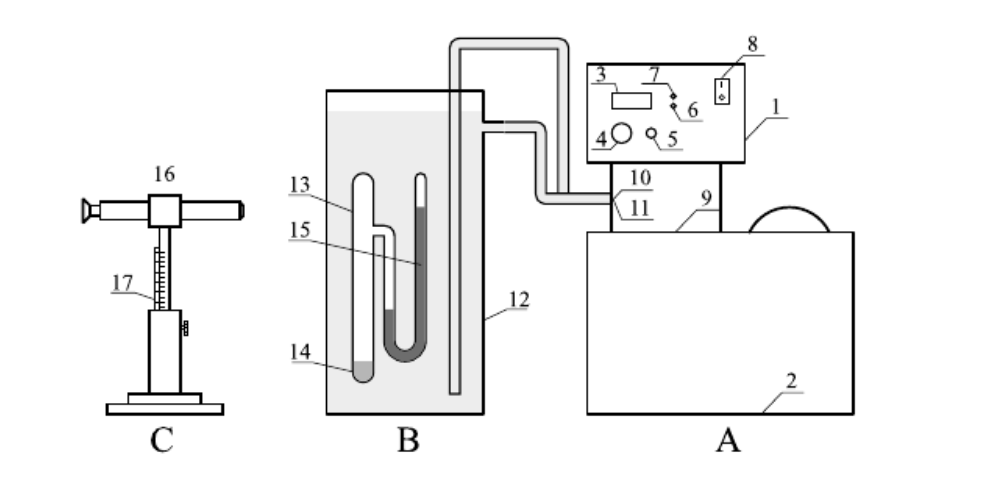
\includegraphics[width = 15cm]{images/installation.png}
        \caption{Схема экспериментальной установки}
        \label{installation}
    \end{figure}

    \noindent Экспериментальный прибор B представляет собой емкость 12, заполненную водой. В нее погружен запаянный прибор 13 с исследуемой жидкостью 14. Перед заполнением исследуемой жидкости воздух из запаянного прибора был удален, так что над жидкостью находится только её насыщенный пар. Давление пара определяется по ртутному манометру 15, соединенному с емкостью 13. Численная величина давления измеряется по разности показаний отсчетного микроскопа 16, настраиваемого последовательно на нижний и верхний уровни столбика ртути манометра. Показания микроскопа снимаются по шкале 17. \\

    \noindent Описание прибора указывает на второе важное преимущество предложенного косвенного метода измерения $L$ перед прямым. При непосредственном измерении теплоты испарения опыты нужно производить при неизменном давлении, и прибор не может быть запаян. При этом невозможно обеспечить такую чистоту и неизменность экспериментальных условий, как при нашей постановке опыта. \\

    \noindent Описываемый прибор обладает важным недостатком: термометр определяет температуру термостата, а не исследуемой жидкости (или ее пара). Эти температуры близки друг к другу лишь в том случае, если нагревание происходит достаточно медленно. Убедиться в том, что темп нагревания не является слишком быстрым, можно, сравнивая результаты, полученные при нагревании и при остывании прибора. Такое сравнение необходимо сделать. Для ориентировки укажем, что температуру воды в калориметре следует менять не быстрее, чем на 1 $^\circ C$ в течение 1–3 минут.

    \section*{Результаты измерений и обработка данных}

    \noindent Для определения теплоты парообразования воды измерим давление насыщенного пара при различных значениях температуры. Давление определяем при помощи ртутного манометра. При помощи штангенциркуля и отсчётного микроскопа находим высоты $h_1$ и $h_2$ ртутных столбиков и находим давление насыщенного пара при определённой температуре по формуле:
    
    \begin{equation}
        \label{P}
        \Delta P = \rho g (h_1 - h_2)
    \end{equation}

    \noindent Результаты измерений заносим в таблицу \ref{tab:measures}. \\

    \noindent При оценке погрешности измерения давления по формуле \eqref{P} следует использовать следующие соотношения:
    \[ \sigma^2_{A\pm B} = \sigma^2_A+\sigma^2_B, \]
    \[ \varepsilon^2_{A\cdot B} = \varepsilon^2_A+\varepsilon^2_B. \]

    \noindent Также на данной установке поверх столбика ртути был столб воды высотой $h' \approx 110,7$ мм. Ввиду значительной высоты столба жидкости следует сделать поправку на это добавочное давление. Занесём в таблицу \ref{tab:measures} скорректированное значение давления насыщенного пара, вычисленное по формуле \[ \Delta P' = \Delta P - \rho_\text{в}gh', \] где $h'$ -- высота столбика воды.

    \begin{table}[H]
        \centering
        \begin{tabular}{|c|c|c|c|c|c|c|c|c|}
        \hline
        $t, ^\circ$C & $T$, K & $\sigma_T$, K & $h_1$, мм & $h_2$, мм & $\sigma_h$, мм & $\Delta P$, Па & $\Delta P'$, Па & $\sigma_{\Delta P'}$, Па \\ \hline
        23,22 & 296,22 & \multirow{18}{*}{0,01} & 110,30 & 83,70 & \multirow{18}{*}{0,01} & 3548,87 & 2462,90 & 0,43 \\ \cline{1-2} \cline{4-5} \cline{7-9} 
        24,09 & 297,09 &  & 110,75 & 83,15 &  & 3682,28 & 2596,31 & 0,46 \\ \cline{1-2} \cline{4-5} \cline{7-9} 
        25,08 & 298,08 &  & 111,30 & 82,70 &  & 3815,70 & 2729,73 & 0,48 \\ \cline{1-2} \cline{4-5} \cline{7-9} 
        26,07 & 299,07 &  & 112,05 & 81,95 &  & 4015,82 & 2929,85 & 0,52 \\ \cline{1-2} \cline{4-5} \cline{7-9} 
        27,09 & 300,09 &  & 112,90 & 81,00 &  & 4255,97 & 3170,00 & 0,56 \\ \cline{1-2} \cline{4-5} \cline{7-9} 
        28,08 & 301,08 &  & 113,85 & 80,00 &  & 4516,13 & 3430,16 & 0,61 \\ \cline{1-2} \cline{4-5} \cline{7-9} 
        29,08 & 302,08 &  & 114,15 & 79,65 &  & 4602,85 & 3516,89 & 0,63 \\ \cline{1-2} \cline{4-5} \cline{7-9} 
        30,08 & 303,08 &  & 115,55 & 78,75 &  & 4909,71 & 3823,74 & 0,68 \\ \cline{1-2} \cline{4-5} \cline{7-9} 
        31,08 & 304,08 &  & 116,75 & 78,05 &  & 5163,20 & 4077,23 & 0,73 \\ \cline{1-2} \cline{4-5} \cline{7-9} 
        32,07 & 305,07 &  & 116,95 & 76,65 &  & 5376,66 & 4290,70 & 0,77 \\ \cline{1-2} \cline{4-5} \cline{7-9} 
        33,07 & 306,07 &  & 118,30 & 75,95 &  & 5650,17 & 4564,20 & 0,82 \\ \cline{1-2} \cline{4-5} \cline{7-9} 
        34,08 & 307,08 &  & 119,40 & 75,00 &  & 5923,67 & 4837,70 & 0,88 \\ \cline{1-2} \cline{4-5} \cline{7-9} 
        35,07 & 308,07 &  & 120,30 & 74,00 &  & 6177,16 & 5091,19 & 0,93 \\ \cline{1-2} \cline{4-5} \cline{7-9} 
        36,06 & 309,06 &  & 122,00 & 72,65 &  & 6584,08 & 5498,11 & 1,01 \\ \cline{1-2} \cline{4-5} \cline{7-9} 
        37,07 & 310,07 &  & 122,60 & 71,65 &  & 6797,55 & 5711,58 & 1,06 \\ \cline{1-2} \cline{4-5} \cline{7-9} 
        38,06 & 311,06 &  & 124,50 & 70,40 &  & 7217,81 & 6131,84 & 1,14 \\ \cline{1-2} \cline{4-5} \cline{7-9} 
        39,07 & 312,07 &  & 125,10 & 69,15 &  & 7464,63 & 6378,66 & 1,20 \\ \cline{1-2} \cline{4-5} \cline{7-9} 
        40,07 & 313,07 &  & 127,80 & 67,55 &  & 8038,31 & 6952,35 & 1,32 \\ \hline
        \end{tabular}
        \caption{Измерение зависимости давления насыщенного пара от температуры жидкости}
        \label{tab:measures}
    \end{table}

    \noindent Отметим, что все измерения проводились только при возрастании температуры термостата вследствие того, что она менялась на 1 $^\circ C$ в течение 5 минут, то есть нагревание происходило крайне медленно.

    \subsection*{Определение теплоты парообразования по графику $ P(T) $}

    \noindent По данным из таблицы \ref{tab:measures} построим график зависимости давления насыщенного пара от температуры (рис. \ref{graph1}). Заметим, что значения погрешностей малы по сравнению с маштабом графика, поэтому кресты погрешности не будут изображены.

    \begin{figure}[H]
        \centering
        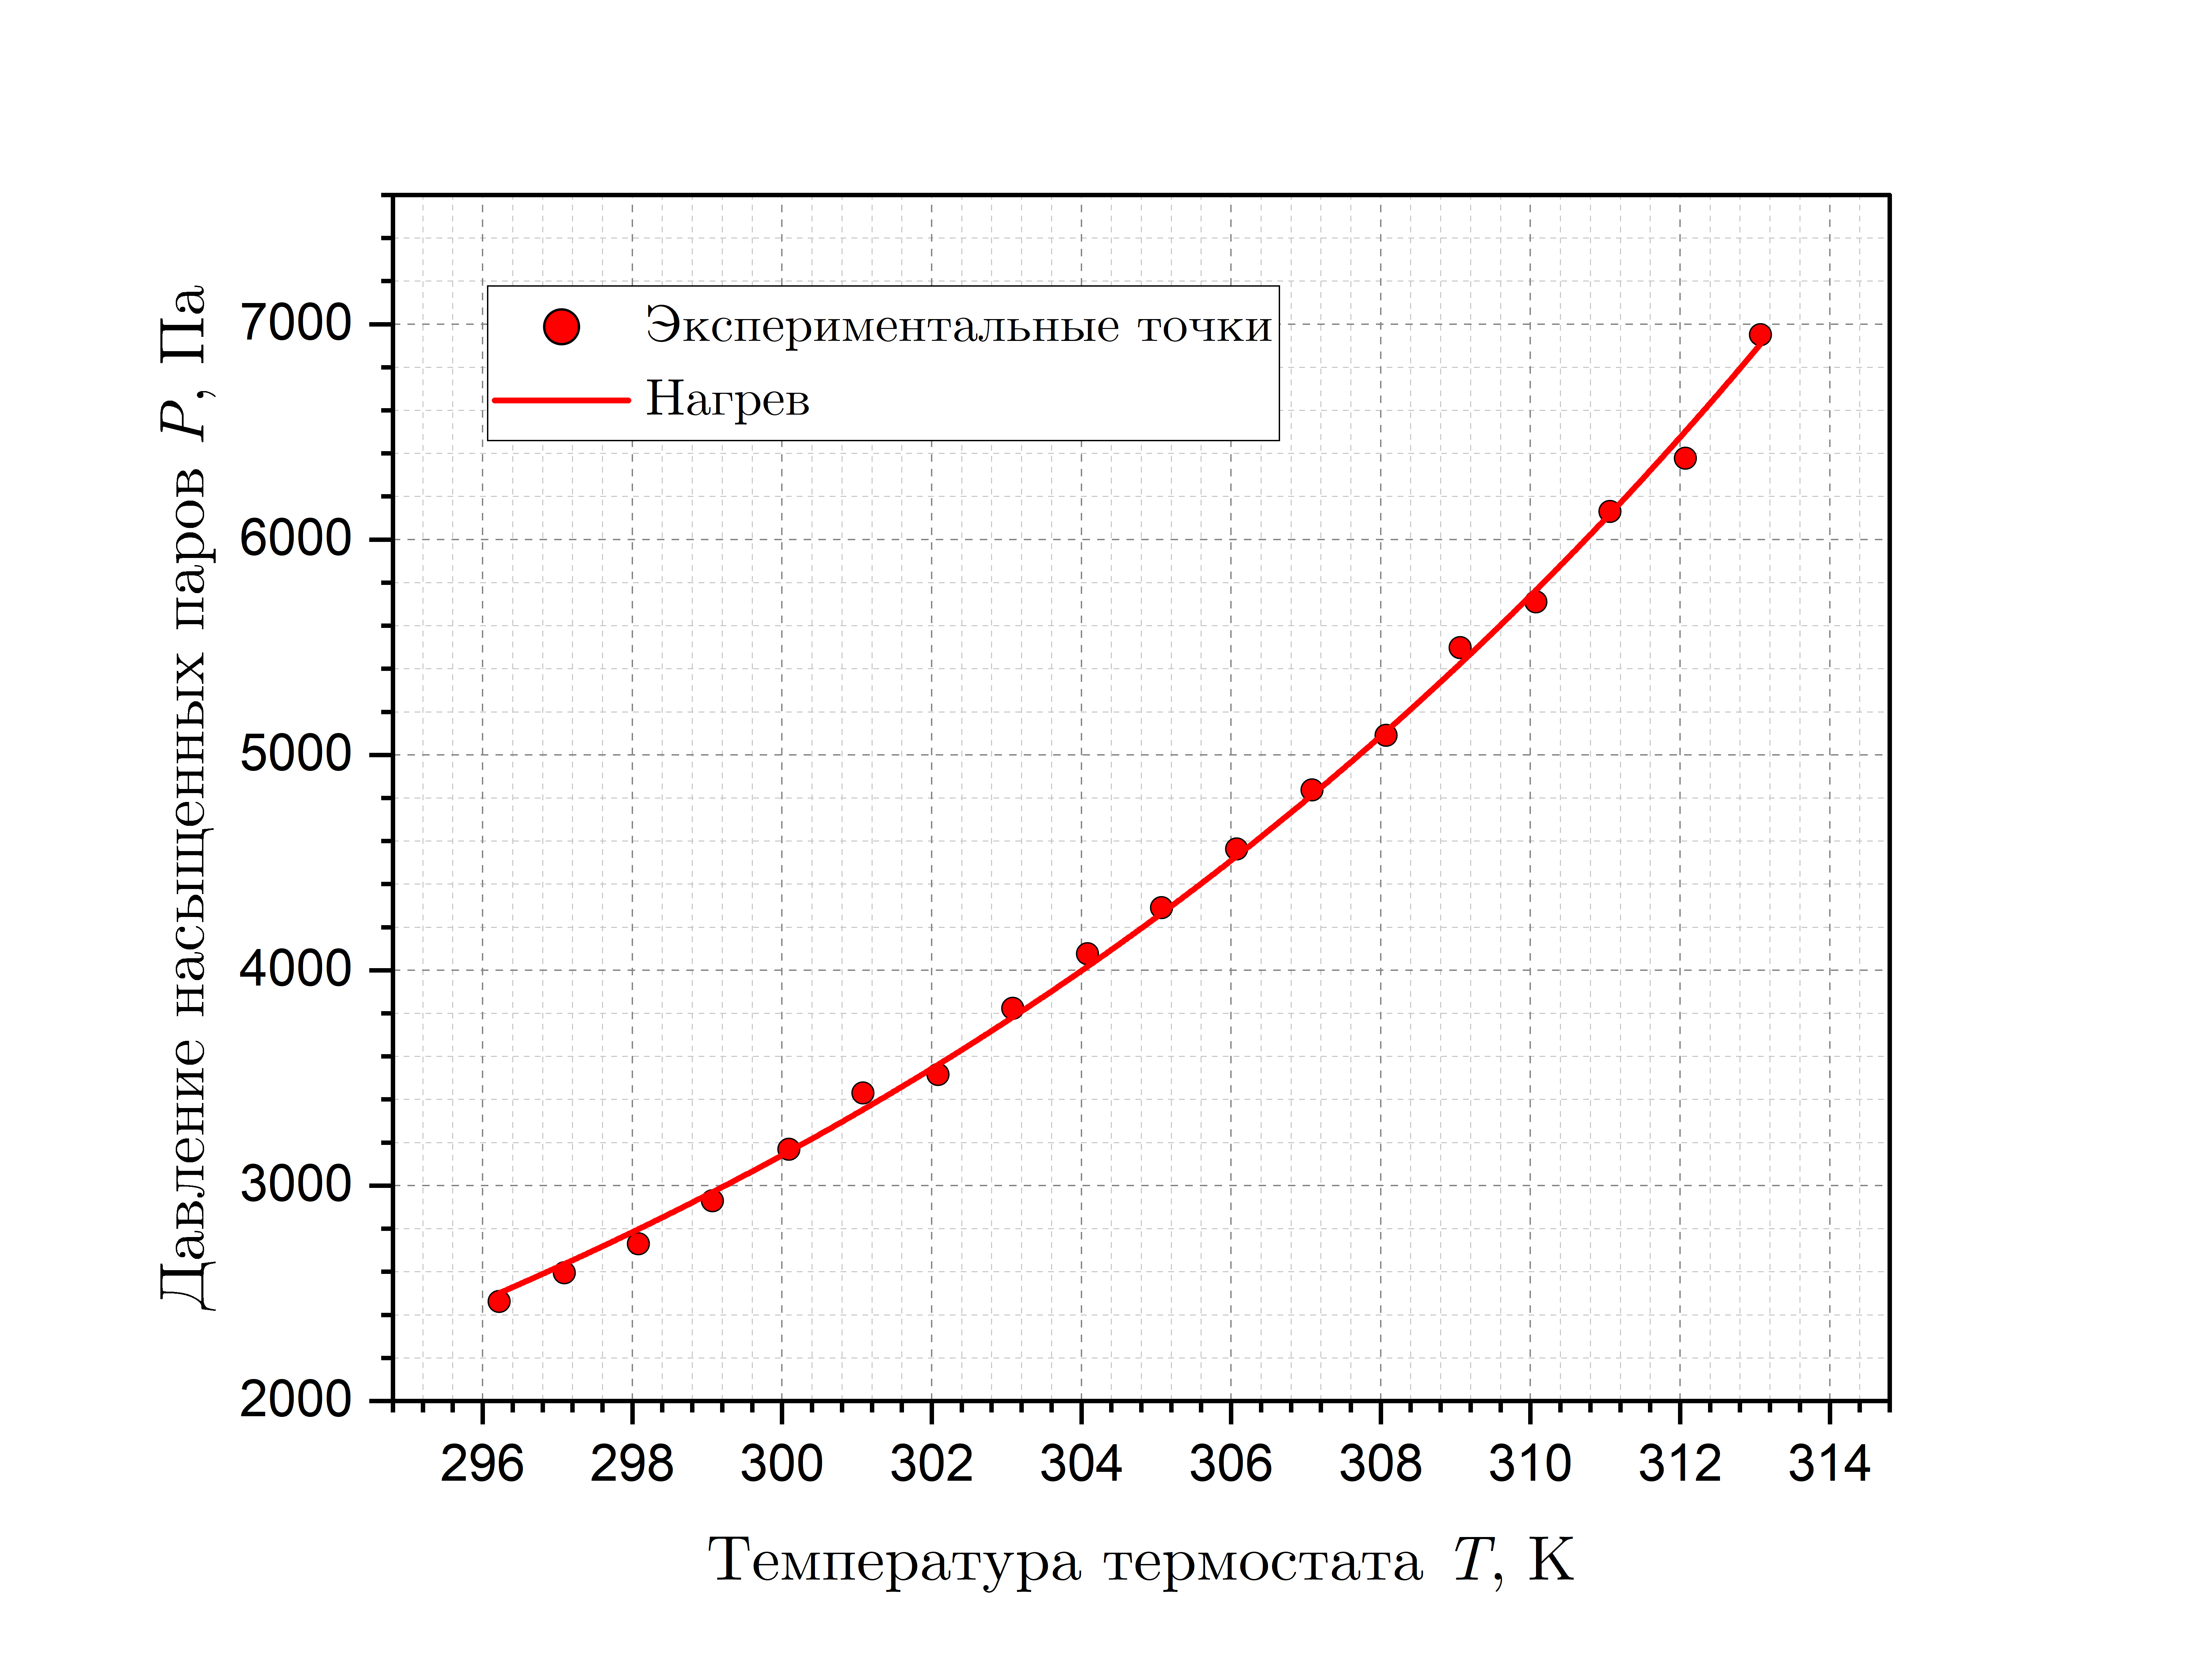
\includegraphics[width = 15cm]{images/P(T).png}
        \caption{График зависимости давления насыщенного пара от температуры термостата}
        \label{graph1}
    \end{figure}

    \noindent Аппроксимируем полученную зависимость в программе \textit{Origin Pro 2023} функциями вида \[ P=ae^{bT}, \] где $a$ и $b$ -- неизвестные параметры. \\

    \noindent Полученные результаты заносим в таблицу \ref{tab:ab} и наносим зависимости на график.

    \begin{table}[H]
	\centering
	\begin{tabular}{|c|c|c|c|c|}
		\hline
            $a \cdot 10^{-5}$, Па & $ \sigma_a \cdot 10^{-5}$, Па & $ b \cdot 10^{-2} $, К$ ^{-1} $ & $ \sigma_b \cdot 10^{-2} $, К$ ^{-1} $ \\ \hline
		4,4 & 0,9 & 6,03 & 0,06 \\ \hline
	\end{tabular}
	\caption{Определение коэффициентов зависимости}
	\label{tab:ab}
    \end{table}

    \noindent Используя полученные результаты, можно получить формулу для производной давления по температуру:
    
    \begin{equation}
        \label{dpdt}
        \frac{dP}{dT} = abe^{bT}.
    \end{equation}
    
    \noindent Подставляя \eqref{dpdt} в \eqref{final}, получаем:
    
    \begin{equation}
        \label{newFinal}
        L=\frac{RT^2ab}{P}e^{bT}.
    \end{equation}

    \noindent По полученным выше формулам вычисляем теплоту парообразования воды. Погрешность вычисления этой величины можно оценить по следующим формулам:
    
    \[ \sigma_L = L\varepsilon_{\frac{dP}{dT}}, \]
    \[ \sigma_{\frac{dP}{dT}} = \sqrt{\left(\frac{\partial\frac{dP}{dT}}{\partial a}\sigma_a\right)^2+\left(\frac{\partial\frac{dP}{dT}}{\partial b}\sigma_b\right)^2} \]

    \noindent Полученные результаты, котоые затем сравним со значениями, полученными  другим методом, заносим в таблицу \ref{tab:par}.

    \begin{table}[H]
        \centering
        \begin{tabular}{|c|c|c|c|}
        \hline
        $T$, K & $P$, Па & $L, \frac{\text{кДж}}{\text{моль}}$ & $\sigma_L, \frac{\text{кДж}}{\text{моль}}$ \\ \hline
        296,22 & 2462,90 & 44,93 & 9,20 \\ \hline
        297,09 & 2596,31 & 45,18 & 9,25 \\ \hline
        298,08 & 2729,73 & 45,92 & 9,40 \\ \hline
        299,07 & 2929,85 & 45,72 & 9,36 \\ \hline
        300,09 & 3170,00 & 45,24 & 9,27 \\ \hline
        301,08 & 3430,16 & 44,68 & 9,15 \\ \hline
        302,08 & 3516,89 & 46,59 & 9,54 \\ \hline
        303,08 & 3823,74 & 45,82 & 9,38 \\ \hline
        304,08 & 4077,23 & 45,94 & 9,41 \\ \hline
        305,07 & 4290,70 & 46,64 & 9,55 \\ \hline
        306,07 & 4564,20 & 46,88 & 9,60 \\ \hline
        307,08 & 4837,70 & 47,32 & 9,69 \\ \hline
        308,07 & 5091,19 & 48,04 & 9,84 \\ \hline
        309,06 & 5498,11 & 47,52 & 9,73 \\ \hline
        310,07 & 5711,58 & 48,94 & 10,02 \\ \hline
        311,06 & 6131,84 & 48,70 & 9,97 \\ \hline
        312,07 & 6378,66 & 50,08 & 10,25 \\ \hline
        313,07 & 6952,35 & 49,11 & 10,06 \\ \hline
        \end{tabular}   
        \caption{Результаты вычисления теплоты парообразования}
        \label{tab:par}
    \end{table}

    \newpage

    \subsection*{Определение теплоты парообразования по графику $\ln P$ от $1/T$}

    \noindent Для построения графика $\ln P (1/T)$ (рис. \ref{graph2}) преобразуем данные из таблицы \ref{tab:measures}. Преобразованные результаты измерений занесём в таблицу \ref{tab:ln}.

    \begin{table}[H]
        \centering
            \begin{tabular}{|c|c|}
            \hline
            $1/T$, $10^{-3} \cdot K^{-1}$ & $\ln P$ \\ \hline
            3,38 & 7,81 \\ \hline
            3,37 & 7,86 \\ \hline
            3,35 & 7,91 \\ \hline
            3,34 & 7,98 \\ \hline
            3,33 & 8,06 \\ \hline
            3,32 & 8,14 \\ \hline
            3,31 & 8,17 \\ \hline
            3,30 & 8,25 \\ \hline
            3,29 & 8,31 \\ \hline
            3,28 & 8,36 \\ \hline
            3,27 & 8,43 \\ \hline
            3,26 & 8,48 \\ \hline
            3,25 & 8,54 \\ \hline
            3,24 & 8,61 \\ \hline
            3,23 & 8,65 \\ \hline
            3,21 & 8,72 \\ \hline
            3,20 & 8,76 \\ \hline
            3,19 & 8,85 \\ \hline
            \end{tabular}
        \caption{Зависимость $\ln P$ от $1/T$}
        \label{tab:ln}
    \end{table}

     \begin{figure}[H]
        \centering
        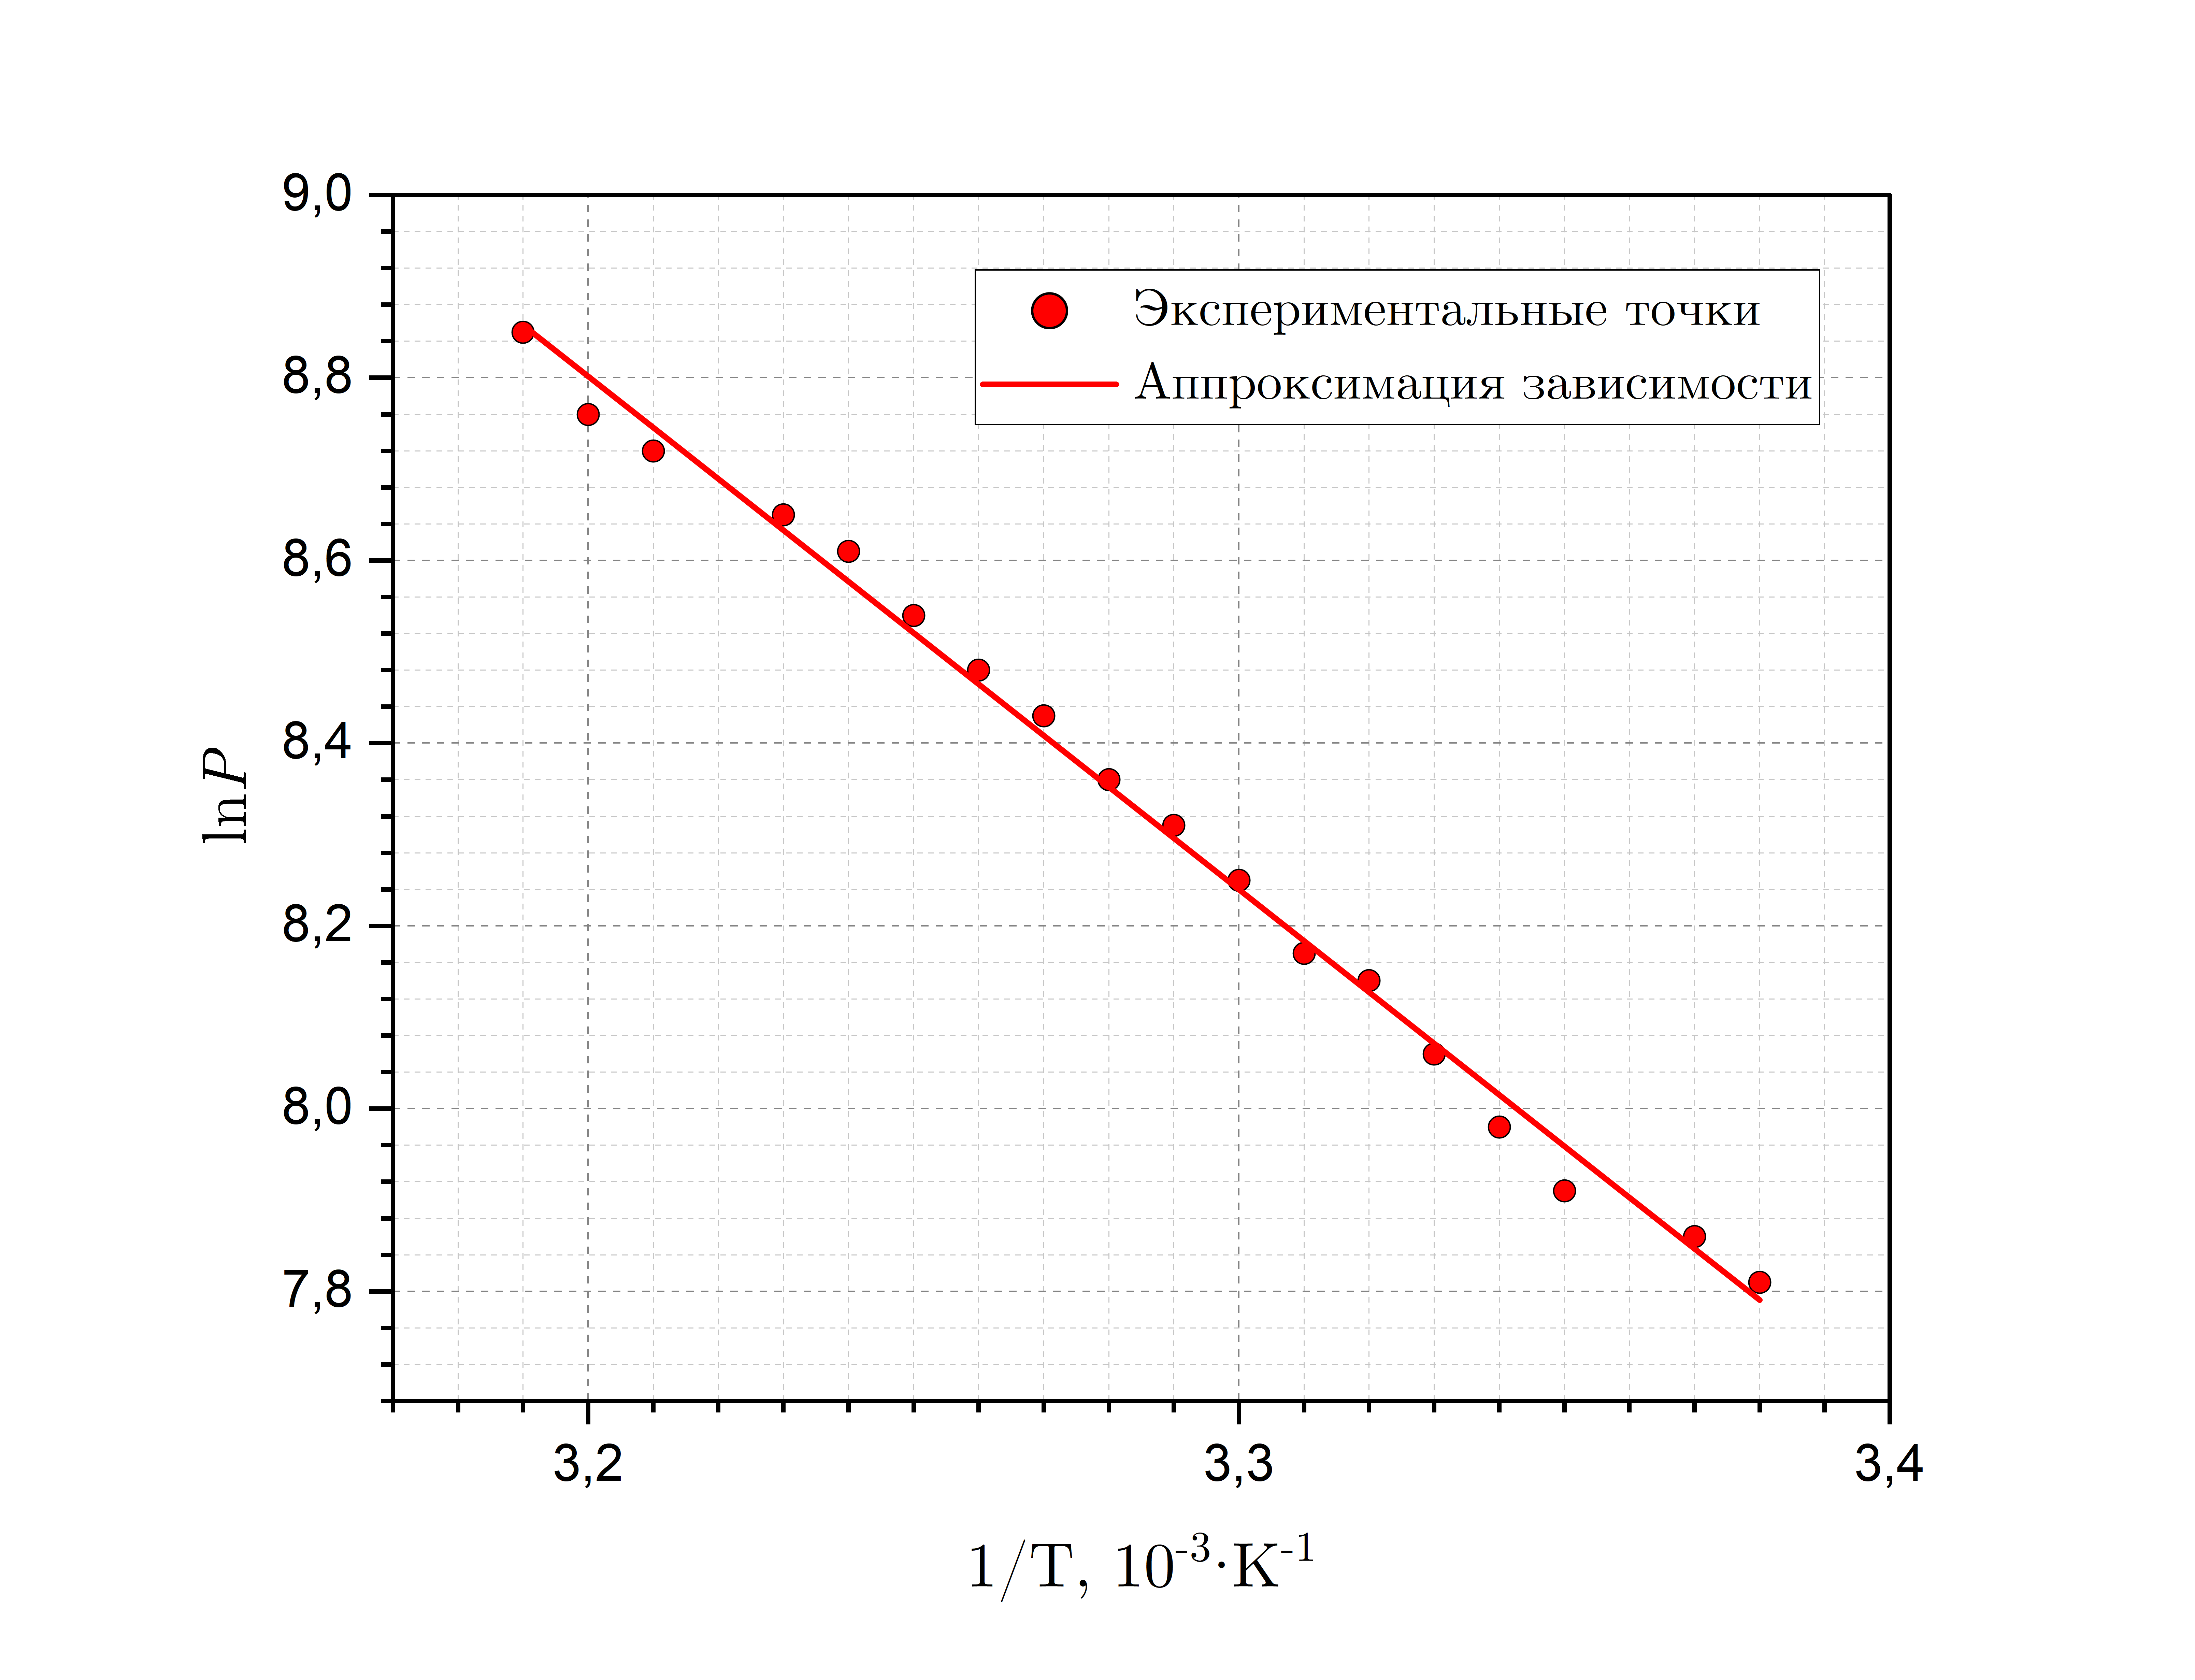
\includegraphics[width = 15cm]{images/lnP.png}
        \caption{График зависимости $\ln P (1/T)$}
        \label{graph2}
    \end{figure}

    \noindent Аппроксимируем полученную зависимость в программе \textit{Origin Pro 2023}, получим:
    
    \[ \frac{d(\ln P)}{d(1/T)} = \left(-5,6\pm 0,1\right) \cdot 10^{3} \text{ К}.\]

    \noindent По формуле \eqref{final} вычисляем теплоту парообразования. Получаем:
    
    \[ \boxed{L = \left(46,5 \pm 0,8\right) \: \frac{\text{кДж}}{\text{моль}} \quad \left( \varepsilon_L = 1,7 \% \right)} \]

    \noindent Полученное значение будет сравнено с эталонным значением и со значениями, полученными в предыдущей части работы.
    
    \section*{Заключение}
    
    \noindent В ходе выполнения работы:

    \begin{itemize}
        \item были вычислены теплоты парообразования воды для различных температур двумя разными способами;
        \item была доказана применимость уравнения Клапейрона-Клаузиуса и верность допущенных в теоретической части работы приближений.
    \end{itemize}

    \noindent Результаты вычисления теплоты парообразования по графику $P(T)$ представлены в таблице \ref{tab:results}.

    \begin{table}[H]
        \centering
        \begin{tabular}{|c|c|c|c|c|}
        \hline
        $ T $, К & $P$, Па & $L$, $\frac{\text{МДж}}{\text{кг}}$ & $\sigma_L $, $\frac{\text{МДж}}{\text{кг}}$ & $\varepsilon $, \% \\ \hline
        296,22 & 2462,90 & 2,50 & 0,51 & 20,0 \\ \hline
        297,09 & 2596,31 & 2,51 & 0,51 & 20,0 \\ \hline
        298,08 & 2729,73 & 2,55 & 0,52 & 20,0 \\ \hline
        299,07 & 2929,85 & 2,54 & 0,52 & 20,0 \\ \hline
        300,09 & 3170,00 & 2,51 & 0,51 & 20,0 \\ \hline
        301,08 & 3430,16 & 2,48 & 0,51 & 20,0 \\ \hline
        302,08 & 3516,89 & 2,59 & 0,53 & 20,0 \\ \hline
        303,08 & 3823,74 & 2,55 & 0,52 & 20,0 \\ \hline
        304,08 & 4077,23 & 2,55 & 0,52 & 20,0 \\ \hline
        305,07 & 4290,70 & 2,59 & 0,53 & 20,0 \\ \hline
        306,07 & 4564,20 & 2,60 & 0,53 & 20,0 \\ \hline
        307,08 & 4837,70 & 2,63 & 0,54 & 20,0 \\ \hline
        308,07 & 5091,19 & 2,67 & 0,55 & 20,0 \\ \hline
        309,06 & 5498,11 & 2,64 & 0,54 & 20,0 \\ \hline
        310,07 & 5711,58 & 2,72 & 0,56 & 20,0 \\ \hline
        311,06 & 6131,84 & 2,71 & 0,55 & 20,0 \\ \hline
        312,07 & 6378,66 & 2,78 & 0,57 & 20,0 \\ \hline
        313,07 & 6952,35 & 2,73 & 0,56 & 20,0 \\ \hline
        \end{tabular}
        \caption{Результаты измерений теплоты парообразования}
	\label{tab:results}
    \end{table}

    \noindent Также теплота парообразования была определена при помощи графика зависимости $\ln P$ от $1/T$. По результатам этих измерений получили:

    \[ \boxed{L = \left(2,58 \pm 0,04\right) \frac{\text{кДж}}{\text{кг}} \quad (\varepsilon_L = 1,7 \%),} \] 

    \noindent Данные, полученные при помощи двух различных методов, находятся в согласии друг с другом. \\

    \noindent Сравним полученные данные с табличными:

    \[ L = 2,26 \text{ } \frac{\text{кДж}}{\text{кг}}. \]

    \noindent В пределах погрешности с табличными данными совпадают результаты измерения теплоты парообразования по графику $P(T)$, но в тоже время, у этого метода большая погрешность вычисления. \\

    \noindent При вычислении теплоты парообразования по графику зависимости $\ln P$ от $1/T$ мы получаем среднее значение для всего исследуемого отрезка температур. Из-за этого у данного метода небольшая погрешность, т.к. происходит усреднение по множеству точек. \\

    \noindent В ходе выполнения работы основной вклад в погрешность определения теплоты парообразования внёс дополнительный столб воды, который образовался сверху столбика ртути на установке, несмотря на то, что дополнительное давление было учтено.

\end{document}